\documentclass[defaultstyle,11pt]{thesis}


% custom added -- must go first
\usepackage[table,xcdraw]{xcolor} % support using rowcolor when pasting from table generator

% default packages from CU Boulder's template
\usepackage{amssymb}		% to get all AMS symbols
\usepackage{amsmath}
\usepackage{graphicx}		% to insert figures
\usepackage{float}
\usepackage{todonotes}
\usepackage{multirow}

% setup hyperlinks and colors
\usepackage{hyperref}		
\hypersetup{
	colorlinks   = true, %Colours links instead of ugly boxes
	urlcolor     = blue, %Colour for external hyperlinks
	linkcolor    = blue, %Colour of internal links
	citecolor   = blue %Colour of citations
}

% custom added
\usepackage{subfiles}
\usepackage{subcaption}
\usepackage[export]{adjustbox}  % allow margin definition in tables (center images)
\usepackage[acronym,toc,nomain]{glossaries}
\loadglsentries{acronyms}
\makeglossaries % for acronyms
\renewcommand*{\glspostdescription}{} % Removes dots at the end of each entry.
\glsnogroupskiptrue % skip spaces in acronym list (that is don't group alphabetically)
\renewcommand*{\glstextformat}[1]{\textcolor{darkgray}{#1}}  % Hyperlink color of glossary links

% column with ragged right and hyphenation
\usepackage{array}
\usepackage{ragged2e}

% table layout settings
\newcolumntype{P}[1]{>{\RaggedRight\hspace{0pt}}p{#1}}
\newcolumntype{L}[1]{>{\RaggedRight\let\newline\\\arraybackslash\hspace{0pt}}m{#1}}
\newcolumntype{C}[1]{>{\centering\let\newline\\\arraybackslash\hspace{0pt}}m{#1}}
\newcolumntype{R}[1]{>{\RaggedLeft\let\newline\\\arraybackslash\hspace{0pt}}m{#1}}
\newcolumntype{M}[1]{>{\RaggedRight\arraybackslash}m{#1}}

% enum hyperlinks
\usepackage{enumitem}

% code highlighting
\usepackage{listings}
%% listings-modelica.cfg
%% Copyright 2014 Martin Sjoelund, Dietmar Winkler
%
% This work may be distributed and/or modified under the
% conditions of the LaTeX Project Public License, either version 1.3
% of this license or (at your option) any later version.
% The latest version of this license is in
%   http://www.latex-project.org/lppl.txt
% and version 1.3 or later is part of all distributions of LaTeX
% version 2005/12/01 or later.
%
% This work has the LPPL maintenance status `maintained'.
%
% The Current Maintainer of this work is Dietmar Winkler
%
% Code repository https://github.com/modelica-tools/listings-modelica
%
% This work consists of the file listings-modelica.cfg

\lstdefinelanguage{modelica}
{
	morekeywords=[1]{
			algorithm,and,annotation,as,assert,block,break,case,class,connect,connector,
			constant,constrainedby,der,discrete,each,else,elseif,elsewhen,encapsulated,
			end,enumeration,equality,equation,expandable,extends,external,failure,final,
			flow,for,function,guard,if,import,in,initial,inner,input,List,local,loop,
			match,matchcontinue,model,not,operator,Option,or,outer,output,package,parameter,
			partial,protected,public,record,redeclare,replaceable,return,stream,
			subtypeof,then,Tuple,type,uniontype,when,while},
	morekeywords=[2]{true, false},
	% Do not make true,false keywords because fn(true,x, false ) shows up as fn(true,x, *false*)
	morekeywords=[3]{optimization,constraint}, % Optimica keywords
	morekeywords=[4]{objective,startTime,finalTime,initialGuess},
	sensitive=true,
	comment=[l]//,
	morecomment=[s]{/*}{*/},
	alsodigit={.,-},
	morestring=[b]',
	morestring=[b]",
}[keywords,comments,strings]

\definecolor{keywordcolor1}{rgb}{0,0,.4}
\definecolor{keywordcolor2}{rgb}{.90,0,0}
\definecolor{keywordcolor3}{rgb}{.4,0,.8}
\definecolor{keywordcolor4}{rgb}{0.5,0,0.5}
\definecolor{stringcolor}{rgb}{0.133,0.545,0.133}
% \definecolor{listingbgcolor}{rgb}{0.95,0.95,0.95}

\lstset{
	breaklines=true,
	language=modelica,
	basicstyle=\ttfamily,
	keywordstyle=[1]\color{keywordcolor1}\bfseries,
	keywordstyle=[2]\color{keywordcolor2},
	keywordstyle=[3]\color{keywordcolor3}\bfseries,
	keywordstyle=[4]\color{keywordcolor4},
	stringstyle=\color{stringcolor},
	%  backgroundcolor=\color{listingbgcolor},
	framexleftmargin=5pt,
	xleftmargin=5pt,
	xrightmargin=5pt,
	showstringspaces=false
}

\newcommand{\code}[1]{\lstinline|#1|}
\newcommand{\modelica}[1]{\lstinline[language=modelica]|#1|}
\lstset{language = modelica,
	basicstyle=\fontsize{9pt}{10pt}\ttfamily}
\renewcommand\lstlistingname{Code}
\renewcommand\lstlistlistingname{Code}
% color for the background of the code snippets
\definecolor{aliceblue}{rgb}{0.94, 0.97, 1.0}

%\DeclareCaptionStyle{listing} []{}
%\captionsetup[lstlisting]{style=listing, labelsep=none}

% landscape pages
\usepackage{pdflscape}
\usepackage{afterpage}

%%%%%%%%%%%%   All the preamble material:   %%%%%%%%%%%%

\title{CU Example Prospectus Document}

\author{First Middle}{Last}

      
\otherdegrees{B.S., University of Colorado, 2016  \\
		M.S., University of Colorado, 2020}

\degree{Doctor of Philosophy}		%  #1 {long descr.}
{Ph.D., Architectural Engineering}		%  #2 {short descr.}


\dept{Department of}			%  #1 {designation}
{Civil, Environmental and Architectural Engineering}		  %  #2 {department name}

\advisor{Gregor Henze, Ph.D, P.E.}				{\normalsize } %  #1 {title}
%{Ph.D., P.E.}																			%  #2 {name}

\reader{Second Advisor , Ph.D.}		    	    %  2nd person to sign thesis
\readerThree{Third Advisor, Ph.D.}	 	      %  3rd person to sign thesis
\readerFour{Fourth Advisor, Ph.D.}		      %  4th person to sign thesis
\readerFive{Fifth Advisor, Ph.D.}		         %  5th person to sign thesis


\abstract{  \OnePageChapter	% because it is very short

What is the purpose of this document
}

\dedication[Dedication]{	% NEVER use \OnePageChapter here.
To my friends and family
	}

\acknowledgements{	\OnePageChapter	% *MUST* BE ONLY ONE PAGE!
	Support Team:
		Amy Allen
		Sourav Dey
		Thibault Marzullo
	}

% \IRBprotocol{E927F29.001X}	% optional!

\ToCisShort	

\LoFisShort	
% \emptyLoF	% use this if there is no List of Figures

\LoTisShort	
% \emptyLoT	% use this if there is no List of Tables

% LIst of listings (i.e., snippets of code)
\LoLisShort
% \emptyLoL	% use this if there is no List of Listings (code chunks)

% List of acronyms
\LoAisShort
% \emptyLoA	% use this if there are no acronyms

%%%%%%%%%%%%%%%%%%%%%%%%%%%%%%%%%%%%%%%%%%%%%%%%%
%%%%%%%%%%%%%%%       BEGIN DOCUMENT...         %%%%%%%%%%%%%%%%%
%%%%%%%%%%%%%%%%%%%%%%%%%%%%%%%%%%%%%%%%%%%%%%%%%

\begin{document}

% path to where the figures are saved
\graphicspath{{\subfix{figures}}}
\input macros.tex

% main content
\chapter{Introduction}
\label{section_introduction}

\singlespacing	

Example document showing the features of this \LaTeX\ class. Citations are similar to any other \LaTeX\ document and require a bibtex format of the bibliography to be saved in the project directory. 

\section{Figures}

Figures have to be saved in a \texttt{figures} as defined in the main \texttt{main-cu-example.tex} file. Figure \ref{fig_commercial_end_uses} shows the breakdown of commercial building energy consumption in the United States \cite{EnergyInformationAdministration2020}.

\begin{figure}[H]
	\begin{center}
		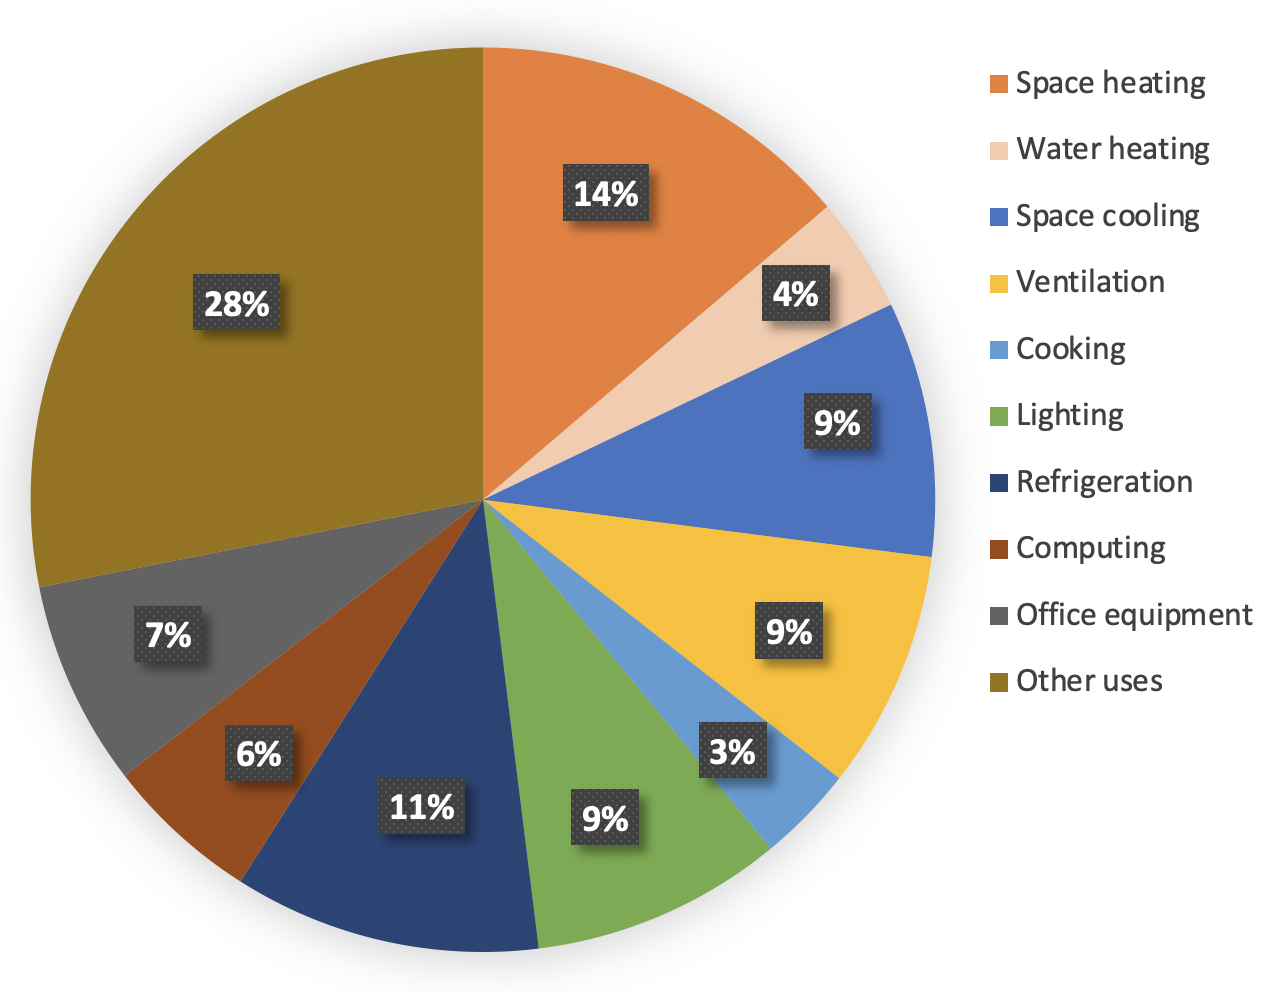
\includegraphics[width=0.5\linewidth]{fig_commercial_end_uses.png}
	\end{center}
	\caption{Commercial building energy use}
	\label{fig_commercial_end_uses}
\end{figure}

If the figure has a citation in it, then make sure to use the ``two level caption" so the citation does not appear in the table of contents. This can cause an issue when the references/citations are shown in the order of appearance. Note the use of square brackets as the first caption.

\begin{figure}[H]
	\begin{center}
		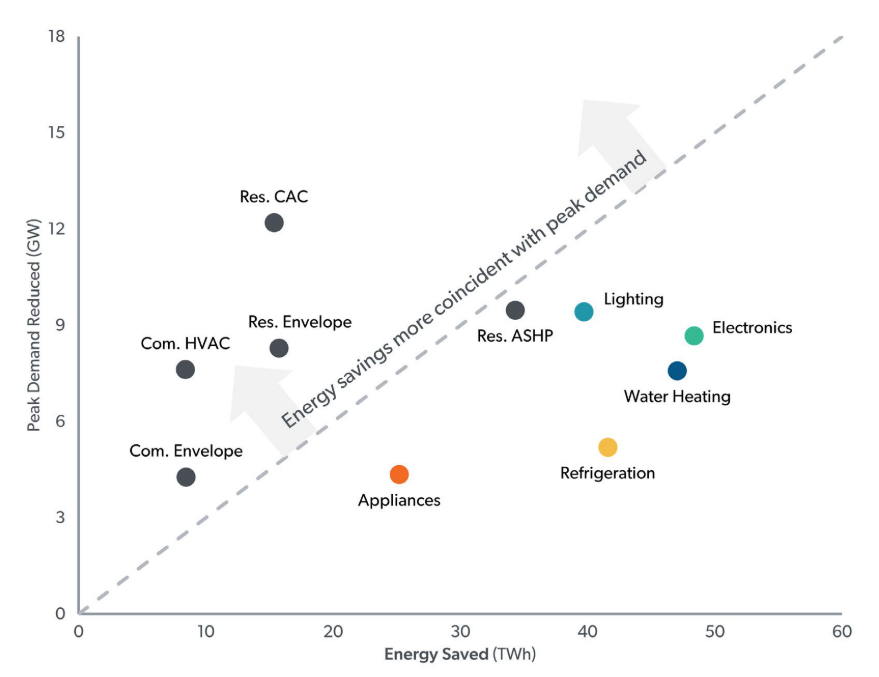
\includegraphics[width=0.5\linewidth]{fig_energy_peak_demand.png}
	\end{center}
	\caption[Peak demand reduction vs energy saved by building technology]{Peak demand reduction vs energy saved by building technology \cite{Satchwell2021}}
	\label{fig_energy_peak_demand}
\end{figure}


\section{Tables}

An example table with caption is shown in Table \ref{tbl_example}.

\begin{table}[H]
	\centering
	\caption{Example table of objectives}
	\begin{tabular}{|L{4.5cm}|L{5.5cm}|L{5.0cm}|}
		\hline
		\rowcolor{lightgray}
		\textbf{Research Objective} & \textbf{Method of Achievement}  & \textbf{Expected Outcome}   \\ \hline \hline
		% next row
		Cell 1 & Cell 2 & Cell 2 \\ \hline
		% next row
		Another cell &
		And another cell with some text wrapping if there is enough text needed for it to wrap based on the fixed width defined in the tabular definition &
		Last cell for this row \\ \hline
	\end{tabular}
	\label{tbl_example}
\end{table}

\section{Equations}

ASHRAE Guideline 14's \cite{Landsberg2014} \gls{CVRMSE} and \gls{NMBE} calculations shown in Equations \ref{eq_cvrmse} and \ref{eq_nmbe}, respectively, as well as $r^2$ and various visual plots generated by the \gls{MMF}.

\begin{equation}
	\label{eq_cvrmse}
	CVRMSE=\frac{1}{\bar{y}}\sqrt{\frac{\sum{(y_i-\hat{y}_i)^2}}{n-1}}
\end{equation}
where $y_i$ is the actual data at timestep, $i$, $\hat{y}_i$ is the modeled (or estimate) of the data at timestep, $i$, $\bar{y}$ is the mean of the actual data, and $n$ is the number of samples.

\bigskip

\begin{equation}
	\label{eq_nmbe}
	NMBE=\frac{\sum{(y_i - \hat{y}_i})}{(n-1) \cdot \bar{y}}
\end{equation}
where $y_i$ is the actual data at timestep, $i$, $\hat{y}_i$ is the modeled (or estimate) of the data at timestep, $i$, $\bar{y}$ is the mean of the actual data, and $n$ is the number of samples.


\section{Acronyms}

This document also demonstrates the use of a glossary to provide acronym definitions. The definitions are stores in the \texttt{acronyms.tex} file. For example, a \gls{DES} will be fully defined the first time, then after \gls{DES} will be an acronym. This is a nice feature because if text moves then \LaTeX\ will handle when to spell out the acronym first. The glossary also allows for pluralization, for example \glspl{GEB} will be defined as plural, but later uses can still be singular. A \gls{GEB} is already defined. Lastly, if the acronym glossary contains more items than defined in the document, it will only show the ones that are used.

\section{Lists and Enumerations}

Example of nested enumeration and lists (also known as itemize in \LaTeX\ speak).

\begin{enumerate}
	\item First item
	\begin{itemize}
		\item Example of just a bullet item
		\item Another item
		\item Last item!
	\end{itemize}

	\item Second numbered item
	\begin{enumerate}
		\item Keep the list going,
		\item With more items,
		\item But now I'm done.
	\end{enumerate}
\end{enumerate}

\section{Code Snippets}

An example of code snippets is shown in Python Code \ref{code_gmt_python} below. The code can be used to generate the updated Modelica source code in Code \ref{code_gmt_modelica}.

\begin{lstlisting}[language=Python, backgroundcolor=\color{aliceblue}, caption={Python snippets of Modelica Builder commands}, captionpos=b, label={code_gmt_python}]
	mofile.rename_component_argument(
		"Buildings.ThermalZones.ReducedOrder.EquivalentAirTemperature.VDI6007",
		"eqAirTempVDI",
		"hConvWallOut",
		"hConWallOut"
	)
	
	mofile.add_connect(
		'port_a', f'{thermal_zone_name}.intGainsConv',
		annotations=['Line(points={{0,100},{96,100},{96,20},{92,20}}, color={191,0,0})']
	)
	
	mofile.add_connect(
		f'{thermal_zone_name}.TAir', 'TAir',
		annotations=[
			'Line(points={{93,32},{98,32},{98,48},{110,48}}, color={0,0,127})'
		]
	)
\end{lstlisting}

% Add in a bigskip between code snippets
\bigskip

\begin{lstlisting}[language=Modelica, backgroundcolor=\color{aliceblue}, caption={Updated Modelica code after Modelica Builder}, captionpos=b, label={code_gmt_modelica}]
	Buildings.ThermalZones.ReducedOrder.EquivalentAirTemperature.VDI6007 eqAirTempVDI(
		aExt=0.5,
		wfGro=0,
		hConWallOut=20.0,
		hRad=5.0,
		n=1,
		wfWall={1.0},
		wfWin={0},
		TGro=285.15) "Computes equivalent air temperature for roof"
		annotation (Placement(transformation(extent={{30,34},{50,54}})));
	
	// ... 
	
	connect(personsConv.port, thermalZoneFourElements.intGainsConv)
		annotation (
			Line(points={{68,-52},{96,-52},{96,20},{92,20}}, color={191,0,0}));
	
	connect(thermalZoneFourElements.TAir, TAir) 
		annotation(
			Line(points={{93,32},{98,32},{98,48},{110,48}}, color={0,0,127}));		
\end{lstlisting}





\chapter{Literature Review}
\label{section_literature_review}

Text TK

\chapter{Methodology}
\label{section_methodology}

Text TK

\chapter{Results and Discussion}
\label{section_results}

\chapter{Conclusions and Future Work}
\label{section_conclusions}

%%%%%%%%%   then the Bibliography, if any   %%%%%%%%%
%bibliographystyle{plain}	% or "siam", or "alpha", etc.

% Use IEEEtr to order based on appearance in document. This will make the citations 
% numbered by the order of appearance.

\bibliographystyle{ieeetr}
%\nocite{*}		% list all refs in database, cited or not

% Change the name of the bibliography file if needed.
\bibliography{bibliography}


%%%%%%%%%   then the Appendices, if any   %%%%%%%%%
\appendix
\chapter{Other Interesting Results}
\label{section_appendix_a}

Text TK

\end{document}

